\chapter{Scattering Theory}
\label{chap:basics}

\section{Scattering Cross-Section}
\label{crosssection}

In a scattering experiment one is interested in a detailed
analysis of the scattering pattern as a function of the
characteristics of the incident beam. Monochromator and collimator
specify direction and energy of the incident radiation.  The
radiation interacts with the sample and receives thereby a
momentum transfer $\hbar \B{Q}$. By this process the radiation
receives beside a direction change also an energy change. The
result is described with the help of a cross-section.

\begin{figure}[htb]
\begin{center}
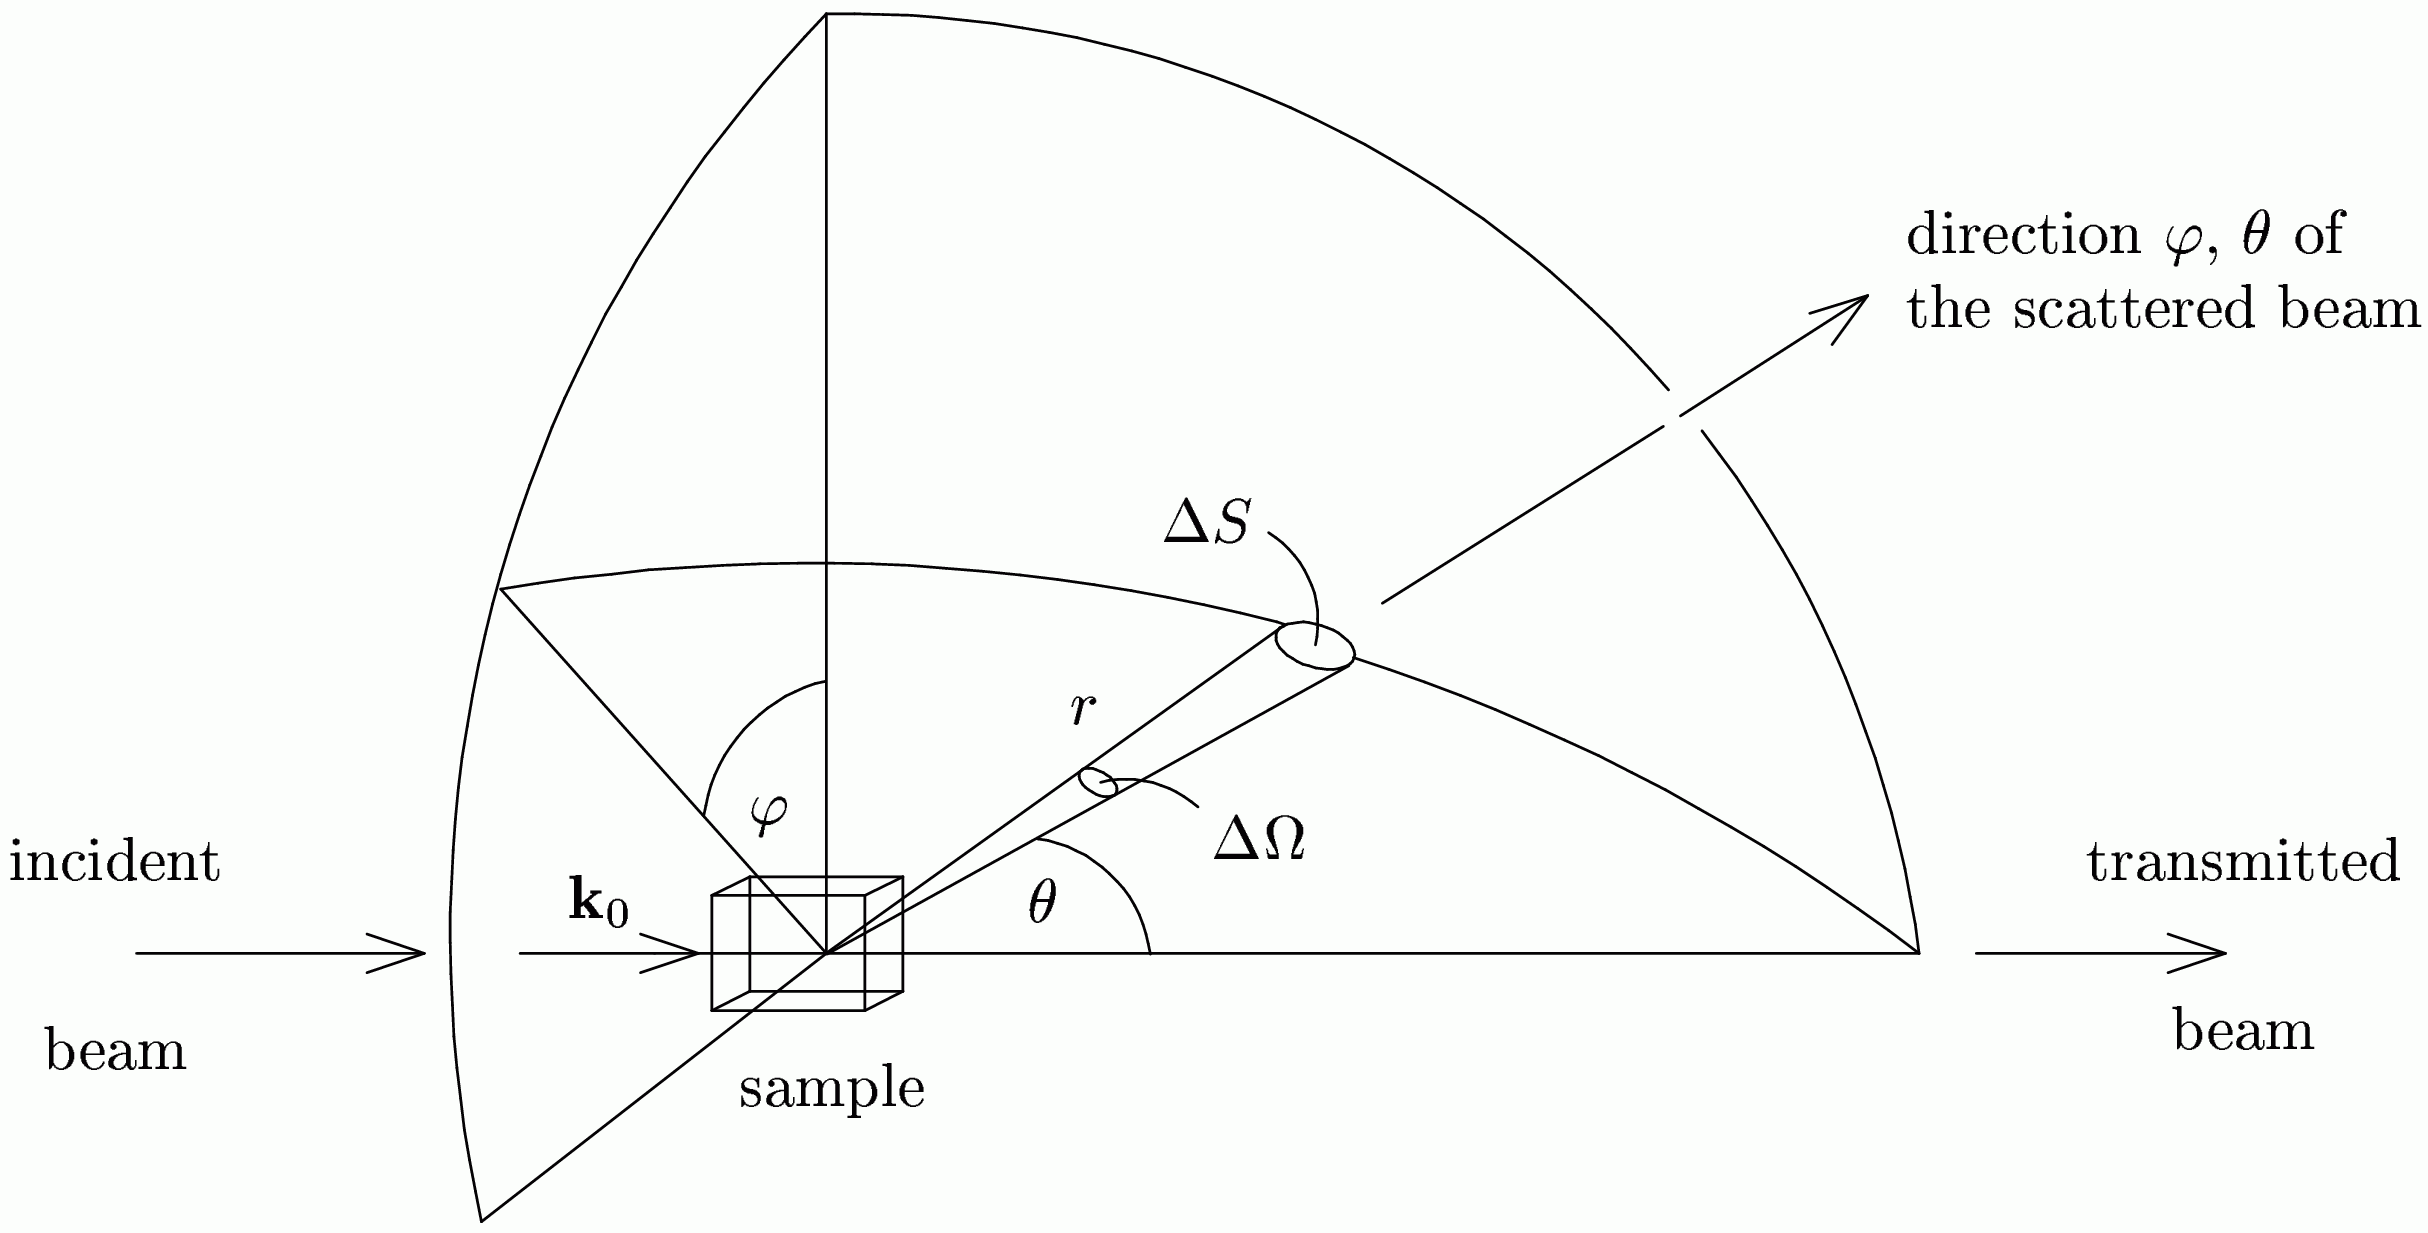
\includegraphics[width=0.9\textwidth,height=0.45\textwidth]{EwaldSphereTeX.png}
\end{center}
\caption{Schematic representation of a scattering process}
\label{scatt2}
\end{figure}

A detector with an efficiency $\epsilon$ measures for this the
number of the scattered neutrons or photons in a given direction
${\bf k}_0+\bf Q$.  The distance between detector and sample
should be large in comparison to the linear dimension of the
detector, so that the solid angle included by the detector element
$\Delta\Omega$ is small.

If the incident beam has a homogeneous, continuous flow
density $\Phi_0$ ($[\Phi_0 ] = $ neutron (photons -) per cm$^2$
and second) and if the beam contain $N$ identical particles, then
the counting rate $C$ of the detector is proportional to all these
quantities. The proportionality constant is called differential
scattering cross-section $ \frac{d\sigma}{d\Omega } =
\frac{C}{\Phi_0 \, \epsilon \, N \, \Delta\Omega } $.  In the case
of inelastic scattering the counting rate is in a certain interval
$\delta E$ of transferred energy in addition proportionally to
$\delta E$. The appropriate proportionality constant is the
partial (or double) differential scattering cross-section
$$
\frac{d^2\sigma}{d\Omega\, dE} = \frac{C}{\Phi_0\, \epsilon\, N\,
\Delta\Omega \,\Delta E } = \rm
\frac{\mbox{\parbox[b]{9.4cm}{\footnotesize Number of neutrons
(photons), which are scattered per second into the solid angle
$d\Omega$ toward $\phi, \theta$ with an energy between $E$ and
$E+dE$}} }{N \Phi_0\, d\Omega\, dE}
$$
The total differential cross-section is defined as
\BE
\sigma_t = (\mbox{total number of scattered neutrons (photons) per sec})/\Phi_0 .
\EE
The three different cross-section are related to each other by
\BE
\sigma_t = \int d\Omega\, \frac{d\sigma}{d\Omega} \qquad \mbox{and}
\qquad \frac{d\sigma}{d\Omega} = \int_0^{\infty}dE\,
                                  \frac{d^2\sigma}{d\Omega\, dE}
.
\EE

\subsection{Scattering of neutrons on atoms}
The scattering of neutrons can be explained by two types of interactions between
neutrons and matter; once the strong spin dependent nuclear forces between nuclei
and neutron (interaction range $\sim 10^{-15}$m) and secondly the dipole-dipole
interaction  between the magnetic moment of the neutron and that of an unpaired electron,
or nuclei accordingly. Both interactions have in common that their interaction potential
$V(\B{r})$ for $r \rightarrow \infty$ decays faster than $1/r$. For this kind of interaction
potential the quantum mechanical scattering theory \cite{hittmair} yields as an asymptotic
approximation for the Schr\"odinger equation of the wave function
\BE \displaystyle
\psi_{\B{k}_0}(\B{r})
\xrightarrow[r\rightarrow\infty]{} \displaystyle
\frac{1}{(2\pi)^{3/2}} \left[e^{\imath\B{k}_0\B{r}} +
f(\theta,\phi)\frac{e^{\imath k_0 r}}{r}\right]
\quad .
\EE
For low energy particles and short range potential the partial waves methods yields for the
scattering amplitude $f(\theta,\phi) = -b$, whereby the so called scattering length $b$ can
be determined experimentally. Via another Ansatz, the Born approximation, one gets a series
expansion for $f(\theta,\phi)$. The first term of this series expansion is give by
\BE \displaystyle
f^{(0)}(\theta,\phi)
= - \frac{m_N}{2 \pi \hbar^2} \int d\B{r}\, e^{\imath\B{Qr}} V(\B{r})
\quad ,
\EE
with $\B{Q} = \B{k-k}_0$. A comparison of this result with the partial wave method
($f(\theta,\phi)=-b$), shows that the pseudo potential
$V(\B{r}) = \frac{2\pi\hbar^2}{m_N} \, b \, \delta(\B{r})$
(Fermi's pseudo potential) has an equivalent solution. For an ensemble of $N$ atoms,
e.g. a crystal, the total potential is in kinematic approximation the sum of the
individual potentials
\BE \displaystyle
V(\B{r}) = \frac{2 \pi \hbar^2}{m_N} \sum_{j=1}^{N} b_j \delta(\B{r-r}_j)
\quad , \label{fermipot}
\EE
whereby $\B{r}_j$ describes the position of nuclei $j$ with scattering the length $b_j$ and $N$
the number of scattering atoms. The scattering length $b_j$ depends on the element or
isotope which is the scattering center. Furthermore it can depend on the spin state of the
neutron and the nuclei and on unpaired electrons in non fully occupied atomic electron shells.
In the kinematic approximation it is assumed that the intensity of the incoming beam is identical
at each scattering center, i.e. that the scattered intensity does not attenuate the incoming beam.
Furthermore it is assumed that the incoming beam is only scattered once and multiple scattered
can be neglected.

In the static approximation, i.e. for a scattering process which does not change the state of the
scattering center and therefore is an elastic scattering process, the differential scattering
cross-section can be described in terms of a scattering amplitude
$f^{(0)}(\theta,\phi)$ by
\BE \frac{d\sigma}{d\Omega}(\B{Q}) = \frac{1}{N}\,
\abs{f^{(0)}(\theta,\phi)}^2 = \frac{1}{N}\, \left(
\frac{m_N}{2\pi\hbar^2}\right)^2 \, \abs{\int d\B{r}\,
e^{\imath\B{Qr}}\, V(\B{r})}^2 \quad . \label{scatteringfunction}
\EE
Using Fermi's pseudo potentials (eq. \ref{fermipot}) leads to the expression
\BE
\frac{d\sigma}{d\Omega}(\B{Q})  = \frac{1}{N} \,
\abs{\sum_{j=1}^N\, b_j\, e^{\imath\B{Qr}_j}}^2  =
 \frac{1}{N}\,\sum_{i,j} b_i\, b_j\, e^{\imath\B{Qr}_i}\, e^{-\imath\B{Qr}_j}
%\\
%&=
%\underbrace{\frac{1}{N}\left( \overline{b^2}-\overline{b}^2\right)
%            }_{\frac{d\sigma_{\rm inc}}{d\Omega}} +
%  \underbrace{\frac{1}{N}\, \overline{b}^2 \, \abs{\sum_i e^{\imath\B{Qr}_i}}^2
%             }_{\frac{d\sigma_{\rm coh}}{d\Omega}}
%\quad .
\label{scatteq1}
\EE

Let us now consider a new system of scatterers, which are only different to those from
eq. \ref{scatteq1} that the scattering length of the nuclei are exchanged. Hereby both
the position and fraction of the scattering length $b_i$ are kept the same.
For a large number of scattering centers the average over the cross-sections of all possible
systems of scatterers which are identical to the one in \ref{scatteq1}
can be described by
\BE
\frac{d\sigma}{d\Omega}(\B{Q}) = \frac{1}{N}\,
                          \sum_{i,j} \overline{b_i\, b_j}\,
                          e^{\imath\B{Qr}_i} \, e^{-\imath\B{Qr}_j}
\qquad . \label{scatteq2}
\EE
If the scattering length $b_i$ occur in the same fraction $x_i$,
whereby $\sum_i x_i = 1$, so that the averages
$\overline{b}$ and $\overline{b^2}$ can be written as
\BE
\overline{b} = \sum_i x_i\, b_i \mbox{~~~ and ~~~}  \overline{b^2} = \sum_i
x_i b_i^2 \quad .
\EE
Under the condition that there are no correlations between the scattering lengths of
the individual nuclei one can write
\BE
\overline{b_i\, b_j} = \overline{b}^2 \mbox{~for~} i \neq j
\qquad \mbox{~and~} \qquad
\overline{b_i\, b_j} = \overline{b^2} \mbox{~for~} i = j
\EE
From this it follows for the differential cross-section
\BE
\frac{d\sigma}{d\Omega}(\B{Q}) = \frac{1}{N} \left( \overline{b^2} +
\overline{b}^2 \sum_{i,j \atop i\neq j} e^{\imath\B{Qr}_i} \,
                                        e^{-\imath\B{Qr}_j} \right)
=
\underbrace{\frac{1}{N}\left( \overline{b^2}-\overline{b}^2\right)
             }_{\frac{d\sigma_{\rm inc}}{d\Omega}} +
  \underbrace{\frac{1}{N}\, \overline{b}^2 \, \abs{\sum_i e^{\imath\B{Qr}_i}}^2
             }_{\frac{d\sigma_{\rm coh}}{d\Omega}}
\EE

\subsubsection{Nuclear scattering}
The simplest system of scatterers consist of only one isotope with nuclear spin $I$.
As the spin of the neutron is $s = \pm 1/2$ only two orientations are possible: parallel
spins of neutron and nuclei, i.e. a total spin of $J_{(+)}=I+1/2$ or antiparallel spins,
i.e $J_{(-)}=I-1/2$.  The corresponding scattering length are named $b_{(+)}$ and
$b_{(-)}$.\footnote{For coherent scattering the spin of the neutrons keep constant in
contrast to incoherent scattering where a part come along with a spin-flip. This can e.g.
be used to change the ration between coherent and incoherent scattering.}

The number of possible states for the total spin $J_{(\pm)}$ are
$2J_{(+)}+1 = 2I+2$ and $2J_{(-)}+1 = 2I$. In case of unpolarized neutrons and/or
random oriented nuclear spins parallel and antiparallel spin states have the same
probability. The fraction $x_{(\pm)}$ of the scattering lengths $b_{(\pm)}$
is therefore proportional to the corresponding number of states
\BE
x_{(+)} = \frac{2J_{(+)}+1}{\left(2J_{(+)}+1\right) + \left(2J_{(-)}+1\right)}
= \frac{I+1}{2I+1} \mbox{~and~} x_{(-)} = \frac{I}{2I+1} \quad .
\EE
For the average scattering length $\overline{b}$ we therefore get
\BE
\overline{b} = \sum_{i=(+),(-)} x_i\, b_i =\frac{1}{2I+1}\left[ (I+1)\, b_{(+)}
+ I\, b_{(-)} \right] \quad .
\EE
For a mixture of different elements and isotopes of type $l$ with nuclear spin $I_l$
and the fraction  $x_l$ (with $\sum_l x_l = 1$) the averages can be written as
\BEA
\overline{b} &=& \sum_l \frac{x_l}{2I_l+1} \left[ (I_l+1)\, b_{l(+)}
+ I_l\, b_{l(-)} \right]  \\
\overline{b^2} &=& \sum_l \frac{x_l}{2I_l+1} \left[ (I_l+1)\,
\left(b_{l(+)}\right)^2
+ I_l\, \left(b_{l(-)}\right)^2 \right] \quad .
\EEA

\subsubsection{Magnetic Scattering}
In magnetic materials the contribution of the interaction between neutrons
and atomic magnetic dipole moments to the scattering length has the same order
of magnitude than the nuclear scattering length. The magnetic scattering is based
on the interaction of the magnetic moment of the neutron $\BM{\mu}_n$ with the magnetic
moment of the scattering atom $\BM{\mu}_A$. The magnetic interaction potential $V(\B{r})$
is described by
\BE
 V(\B{r}) = -\BM{\mu}_n \cdot \B{B}(\B{r}),
\EE
whereby $\BM{\mu}_n=\gamma\frac{e \hbar}{2 m_p}\BM{\sigma}=\gamma\BM{\mu}_N$ is the magnetic dipole
moment\footnote{neutron magnetic moment: $\mu_n=-0.966 236 45 \times 10^{-26}$ JT$^{-1}$,
 neutron magnetic moment to Bohr magneton ratio:$\mu_{\rm n}/\mu_{\rm B}=-1.041 875 63 \times 10^{-3}$,
nuclear magneton: $\mu_{\rm n} = 5.050 783 43 \times 10^{-27}$ JT$^{-1}$,
Bohr magneton: $\mu_{\rm B}=\frac{e\hbar}{2m_e}=927.400 949 \times 10^{-26}$ JT$^{-1}$,
proton mass: $m_p=1.672 621 71 \times 10^{-27}$ kg,
neutron mass: $m_{\rm n}$: $1.674 927 28 \times 10^{-27}$ kg,
electron mass: $m_{\rm e} 9.109 3826 \times 10^{-31}$kg,
elementary charge: $e=1.602 176 53 \times 10^{-19}$ C,
Planck constant over $2\pi$: $\hbar=h/2\pi=1.054 571 68 \times 10^{-34}$ J s}  of
the neutron, \BM{\sigma} Pauli's spin operator, $\gamma$ the
neutron magnetic moment to nuclear magneton
ratio\footnote{neutron magnetic moment to nuclear magneton ratio $\gamma = \mu_{\rm n}/\mu_{\rm N}-1.913 042 73$}
and $\B{B}(\B{r})$ the magnetic field of an atom at the position of the neutron.
An atom generates a magnetic field due to the magnetic dipole moment $\BM{\mu}_S$ of its
electrons $\B{B}_S(\B{r})$
\BE
\B{B}_S(\B{r}) = \BM{\nabla} \times \B{A} \U{~with~} \B{A} =
\frac{\mu_0}{4\pi}\, \frac{\BM{\mu}_S \times\B{r}}{r^3}
\EE
and due to the orbital angular momentum of the electrons $\B{l} = -\B{p}\times\B{r}$
which generates a field of $\B{B}_L(\B{r})$
\BE
\B{B}_L(\B{r}) = -\frac{\mu_0}{4\pi}\, \frac{2\mu_B}{\hbar}\,
\frac{\B{p}\times\B{r}}{r^3}.
\EE
The magnetic interaction potential
$V(\B{r}) = -\BM{\mu}_n\cdot(\B{B}_S(\B{r})+\B{B}_L(\B{r}))$
is a weak long range potential which also can be treated with
Born's approximation.
Compared to the nuclear scattering amplitude the corresponding magnetic scattering
amplitude $b_M$ is given by the Fourier transformation of the magnetic interaction potential
$\mathcal{F}[V(\B{r})]$
\BE
b_M = -\frac{m_n}{2\pi\hbar^2}\, \BM{\mu}_n \cdot \int d^3r \,
e^{\imath\B{Qr}}\, (\B{B}_S(\B{r})+\B{B}_L(\B{r})).
\EE
The Fourier transformation of the magnetic field is related in case of a static magnetic field
to the Fourier transformation of the local magnetization
 $\B{M}(\B{Q}) = \mathcal{F}[\B{M}(\B{r})]$ \cite{book:Squires} by
\BE
\B{B}(\B{Q}) = \mu_0\, \frac{\B{Q}\times [\B{M}(\B{Q})\times\B{Q}]}{Q^2}
             = \mu_0\, \B{M}_{\bot}(\B{Q}),
\EE
whereby $\B{M}_{\bot}(\B{Q})$ is the component of $\B{M}(\B{Q})$ perpendicular to $\B{Q}$ and
$\mu_0 = 4\pi\, 10^{-7}$ Vs/Am the magnetic constant. For the magnetic scattering
amplitude\footnote{Frequently the magnetization is given in units of Bohr magnetons
($\mu_B=\frac{e\hbar}{2m_e}=927.400 949 \times 10^{-26}$ J/T, 1[J/T]=1[Am$^2$])
per atomic volume $\Omega$ so that the magnetic scattering length density can be written as $b_M=D_{\mu}\sum_i c_i{M_i}/\Omega_i$ with
$D_\mu=2.69914\times 10^{-15}$m$^2$. The two constants are related via $D_\mu=D_M\mu_0\mu_B$.} $b_M$
we find than
\BE
b_M = D_M\, \mu_0\, \mbox{\boldmath$\sigma$}\cdot \B{M}_{\bot}(\B{Q})
\mbox{~ with ~} D_M = -\gamma\, \frac{m_n}{2\pi\hbar^2}\, \mu_N = 2.31605 \times
10^{14} \, \frac{1}{\mbox{m$^2$ Tesla}}. \quad
\EE
For scattering on magnetic structures always two interactions have to be considered,
nuclear scattering which is caused by fluctuations in the number density and composition
and magnetic scattering caused by fluctuations in amplitude and/or orientation of the local
magnetization. In case of a preferred orientation, e.g. the direction of an external applied
magnetic field $\B{H}$, the magnetic scattering depends on the spin state {\boldmath $\sigma$}
of the neutron. If $\B{e}_x$ describes the direction of the preferred axis and ($+$) and ($-$)
the neutron spin polarisation antiparallel and parallel to $\B{e}_x$ than the scattering can
be described by four scattering processes; these are two spin non-flip ($++$,$--$) and two
spin flip ($+-$,$-+$) processes. Moon, Riste und Koehler \cite{scatt91} have shown that for
coherent scattering the four scattering length are given by
\BEA
b_{\pm\pm} &= b_N \mp D_M\, \mu_0\, M_{\bot x} \label{eq:Spin:pmpm}\\
b_{\pm\mp} &= - D_M\, \mu_0\, (M_{\bot z} \pm \imath \, M_{\bot
y}).
\EEA
whereby $b_N$ is the nuclear scattering length. In case of unpolarized neutrons the
differential scattering cross-section can be written as
\BE
\frac{d\sigma_{\rm unp}}{d\Omega}(\B{Q}) =
         \frac{d\sigma_{\rm nuc}}{d\Omega}(\B{Q})
       + \frac{d\sigma_{\rm mag}}{d\Omega}(\B{Q}) ,
\EE
because $(b_{++}^2+b_{--}^2+b_{+-}^2+b_{-+}^2)/2 = b_N^2+D_M^2
\mu_0^2 M_{\bot}^2$. For unpolarized neutrons the interference contribution only has
an influence on the degree of polarization of the scattered neutrons but not on the scattering
intensity.
~\\

\subsection{Scattering of x-ray at atoms}

The scattering of x-rays on matter practically exclusively depends on the interaction
of the incoming radiation with electrons. The contribution on the nuclei is negligible small
because the mass of the nuclei is more than $10^3$ times larger than the mass of an electron and
the energy of the nuclear scattering more than $10^6$ smaller than the energy of the scattering
on electrons.

The frequency $\nu_0 = c/\lambda$ of the incoming x-ray beam is in general large against
the resonance frequency of the electrons. In this case the electrons can be considered to be
free and the special properties of the chemical binding are of no importance. These are the conditions
for Thomson-scattering. J.J. Thomson developed a simple classical model for this type of scattering.
Under the influence of an electric field of x-rays electrons start to oscillate. For an incoming plane
and monochromatic wave with an electric field $\B{E} = \B{E}_0 e^{\imath (\B{k}_0\B{r} -
\omega t)}$ the amplitude $E_s$ of a wave scattered on a free electron is
\BE
E_s = -E_0 \frac{e^2}{m_e c^2} \frac{1}{r} \sin \psi .
\EE
Hereby $e$ and $m_e$ are the
charge\footnote{$e = 1.602 176 53 \times 10^{-19}$ C} and
mass\footnote{$m_e = 9.109 3826 \times 10^{-31}$ kg} of the electron, respectively. $c$ is the speed of light\footnote{$c = 299 792 458$ m s$^{-1}$},
$r$ the distance between sample and detector and $\psi$ the angle between the direction of the accelerated
electrons by the incoming wave and the direction of the scattered wave.

Analogously to the neutron scattering length for an electron the x-ray scattering length
(far field of a Hertz dipole) is defined as
\BE
b_{\rm x-ray} = \frac{e^2}{m_e c^2} \sin\psi = r_0 \sin\psi
\EE
whereby $r_0 = e^2 / (m_e c^2) = 2.82 \times 10^{-13}$ cm is the classical electron radius.
For small angle scattering $\psi \simeq \pi/2$ whereby the angle dependent polarization factor is
approximately 1.

For calculating the scattering amplitude of an atom with $Z$ electrons one has to sum up
the scattered waves from the different electrons with the correct phase.
To do this an electron density distribution $\rho_e(\B{r})$ can be introduced which describes the time average
probability distribution of the electron in the atom. The scattering amplitude of an atom is than
\BE
 f_a(\B{Q}) = r_0\, \underbrace{L(Q)}_{{\rm {polarization\atop {factor}}}\sim 1}
\int d\B{r} \, \rho_e(\B{r})\, e^{\imath \B{Qr}}
\stackrel{Q\rightarrow 0}{=} r_0\, Z. \label{diffx}
\EE
The charge distribution in an atom can be described in good approximation by a radial symmetric
function so that
 \BE
f_a(Q) = r_0 \int_0^{\infty} \frac{\sin Qr}{Qr} \, \rho_e(r) \,
4\pi r^2\, dr  \stackrel{Q\rightarrow 0}{=} r_0 \int_0^{\infty}
\rho_e(r) \, 4\pi r^2\, dr  = r_0 Z . \label{diffx}
\EE
In small angle scattering the scattering length of an atom is therefore
$f_a = r_0 Z$ or in units of "electon units [e.u.]" $f=f_a/r_0=Z$.
~\\

\subsubsection{Anomalous scattering of x-rays}

The relation $f=Z$ for atomic scattering length is only valid as long as the energy of the incoming radiation
is much larger than the energy of the K-, L-, etc. shells. In case that the absorption edge of an atom is close
to the energy of the incoming beam the scattering length has to be corrected by a dispersion term.
In general the scattering length of an atom depends on the energy of the x-rays and is a complex number
\BE
f(E) = Z + f'(E) + \imath f''(E) \quad .
\EE
The correction terms $f'$ and $f''$ change the scattering length $f$ near a
K$_{\alpha}$ absorption edge typically up to 30\%.
Figure \ref{fpfppsketch} shows the energy dependency of the scattering length of iron
$f'_{\rm Fe}$ und $f''_{\rm Fe}$.
The dispersion terms are related via the Karamer-Kronig relation
\BE
f'(E) = \frac{2}{\pi}\, \int_0^{\infty} dE'\,
        \frac{E'\, f''(E')}{E'^2-E^2}.
\label{KramerKronig}
\EE
\begin{figure}[htb]
\begin{center}
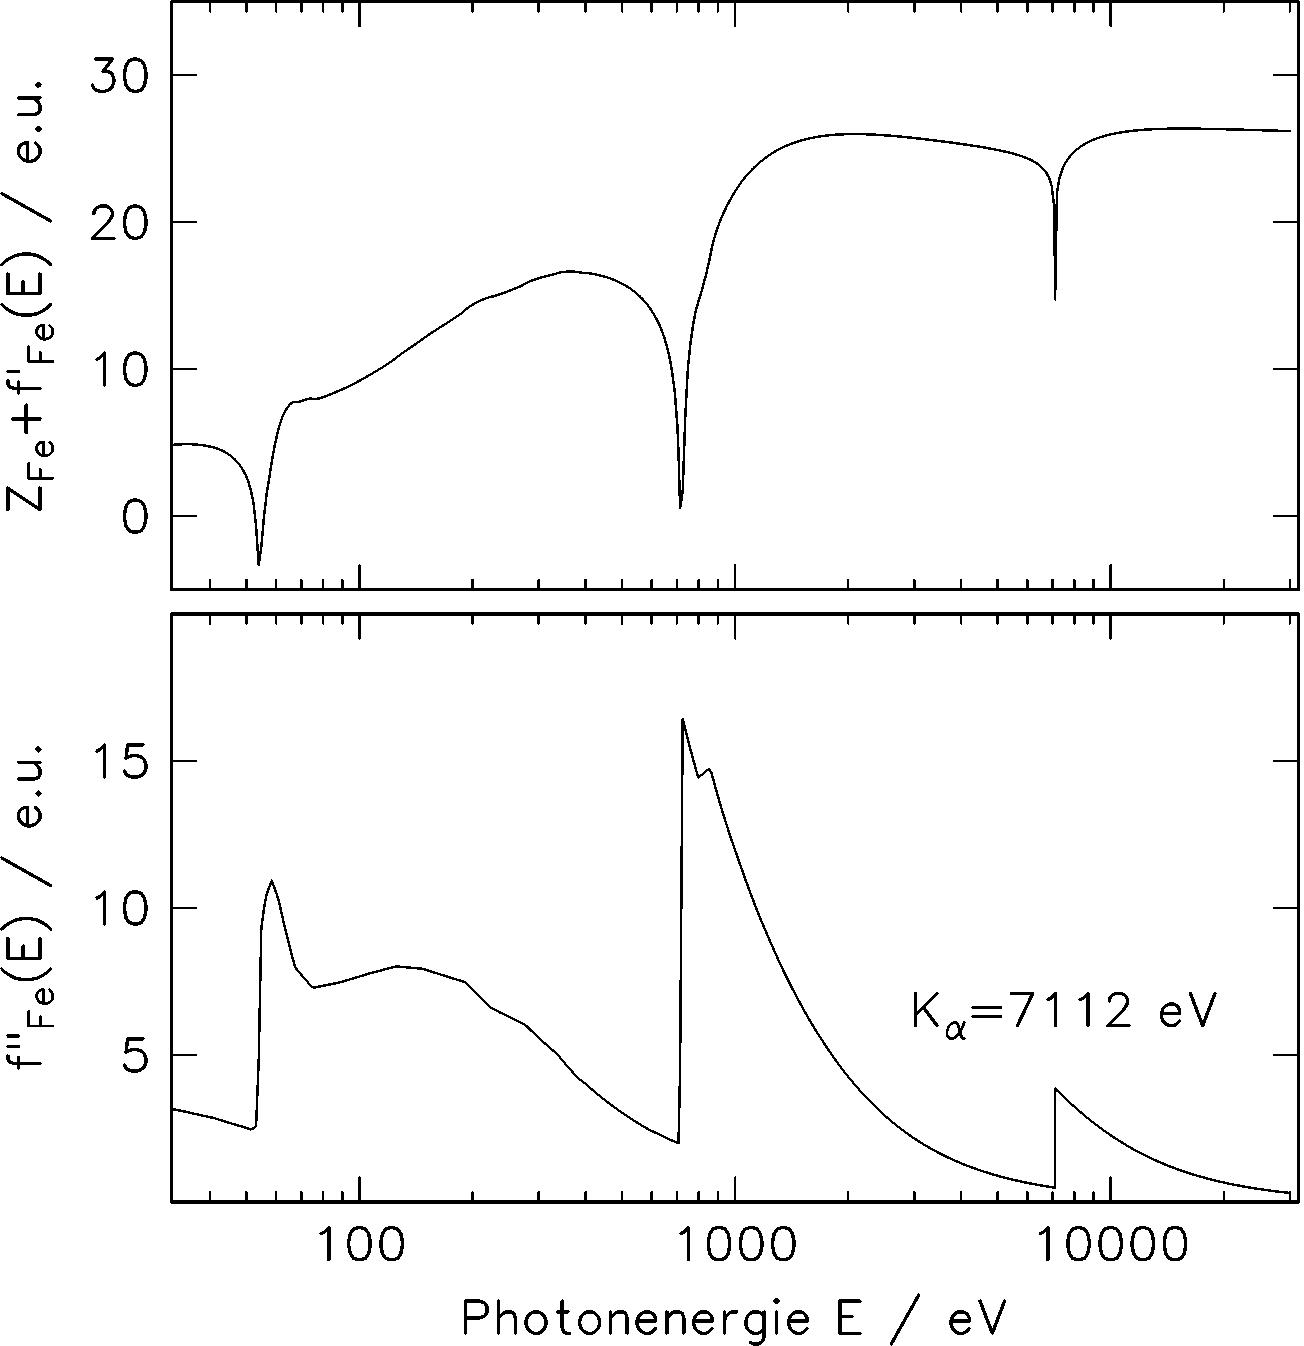
\includegraphics[width=0.7441\textwidth,height=0.7858\textwidth]{FEFPFPP.png}
\caption{Energy dependence of the real and imaginary part of the scattering length of iron:
$Z_{\rm Fe}+ f'_{\rm Fe}(E)$ and $f''_{\rm Fe}(E)$ ($Z_{\rm Fe}=26$)}
\label{fpfppsketch}
\end{center}
\end{figure}
In general the imaginary part $f''$ can be determined experimentally by the mass absorption
coefficient $\mu_m(E)=\frac{2N_A}{A}\, \lambda\, r_0\, f''(E)$ ($N_a$ Avogadro number, $A$
mass of atom in resonance) to calculate than with equation \ref{KramerKronig} the real part of the
scattering length $f'(E)$.

\section{Small angle scattering}

In small angle scattering geometry the structural unit down to single atoms can not be resolved,
only structures larger than several atomic layers can be seen by that method. Small angle
scattering techniques measure the beam scattered close to forward direction whereby the beam
divergence is in the order $\lambda/L \ll 1$. For a wavelength of  $\lambda = 1$ nm and
a characteristic dimension $L = V^{1/3}$ of the scatterer of about 10 nm the divergency of the beam
is  about $\lambda/L = 0.1 \mbox{ rad} \simeq 6.3^{\circ}$.

In principle with small angle scattering  both information on size as well as shape of the scatterer
and information on the relative arrangement of the scatterer can be obtained. In the following an
overview of the theoretical basics to analyze small angle scattering data will be given.

In section \ref{crosssection} the scattering of an ensemble of atoms has been discussed. There
interference terms between the waves scattered by the individual atoms were important for the
differential scattering cross-section (eq. \ref{scatteq1} ,\ref{diffx}).
\BE
\frac{d\sigma}{d\Omega}(\B{Q}) = \frac{1}{N} \, \abs{\sum_{j=1}^N\, b_j\,
e^{\imath\B{Qr}_j}}^2 \qquad \U{or} \qquad
\frac{d\sigma}{d\Omega}(\B{Q}) = \frac{1}{N} \abs{\sum_{j=1}^{N}
f_{a,j}(\B{Q})\, e^{\imath\B{Qr}}}^2  .
\EE
Small angle scattering normally does not resolve dimension down to atomic dimensions.
Therefore the summation over the individual atoms can be replaced by an integration
over the illuminated volume $V$:
\BE
\frac{d\sigma}{d\Omega}(\B{Q}) = \frac{1}{N}\, \abs{\int_V d\B{r}\,
\rho(\B{r})\, e^{\imath \B{Qr}}}^2 = \frac{1}{N}\, I(\B{Q}) \quad ,
\label{scatteq3}
\EE
whereby $\rho(\B{r})$ is the local scattering length density and $F(\B{Q})$
the scattering amplitude. The differential scattering cross-section is mathematically
the square of the modulus of the Fourier transformation of the scattering length density.
The scattering length density $\rho(\B{r})$ is proportional to the locally averaged
scattering potential $\bar V(\B{r})$. Thats why equation \ref{scatteq3} is except a constant
identical to equation \ref{scatteringfunction}. The scattering intensity
$I(\B{Q}) = \abs{z}^2 = z\, z^*$ can therefore be written as
\BE
I(\B{Q}) = \int \!\!\! \int d\B{r}_1\, d\B{r}_2\, \rho(\B{r}_1) \, \rho^*(\B{r}_2)
\, e^{\imath\B{Q(r_{\rm 1}-r_{\rm 2})}} \quad .
\EE
By using the substitution $\B{r} = \B{r}_1 - \B{r}_2$ one get
\BE
I(\B{Q}) = \int d\B{r} \, e^{\imath\B{Qr}}
\underbrace{ \int d\B{r}_1\, \rho(\B{r}_1) \,
\rho^*(\B{r}_1-\B{r}) }_{\displaystyle \Gamma(\B{r}) =  \rho(\B{r}) \circledast
\rho(\B{r}) } = \int d\B{r}\, \Gamma(\B{r})\, e^{\imath\B{Qr}}
\quad . \label{Gamma}
\EE
$\Gamma(\B{r})$ is the autocorrelation function\footnote{Normally
 the autocorrelation function is defined as
 $\rho (\B{r}) \circledast \rho (\B{r}) = \int\, d\B{r}_1\, \rho (\B{r}_1)\,
\rho^{*}(\B{r}_1+\B{r})$, so that in fact $\Gamma (\B{r})$ should be
 $\Gamma (\B{r}) = \rho(-\B{r}) \circledast \rho (-\B{r})$.}
 In case of a real scattering length density eq. \ref{Gamma} is the convolution integral
 $\Gamma(\B{r}) = \rho (\B{r}) * \rho (\B{r}) = \int\, d\B{r}_1\, \rho
(\B{r}_1)\, \rho (\B{r}_1-\B{r})$ of the scattering length density and is called
 Patterson function\footnote{Here the Patterson function is defined as the autocorrelation
 of the scattering length density $\rho(\B{r})$. Instead of defining the cross-section via
 a scattering length density as in \ref{Gamma} in neutron scattering the differential
 cross-section is often defined as
  ${d\sigma_{\rm coh}(\B{Q})}/{d\Omega} = ({\sigma_{\rm coh}}/{4 \pi\,N})\, \int
d\B{r}\,  \rho(\B{r}) \circledast \rho(\B{r})
\,\exp(\imath\B{Q}\B{r})$, whereby $\sigma_{\rm coh} = 4 \pi\,
\overline{b}^2$ is the coherent cross-section and
$\rho(\B{r})$ the particle number density. The Patterson function
is than the autocorrelation of the particle number density. This function is independent
of the scattering lengths and only dependent on the geometric arrangement of the scattering
centers. The Fourier transformation of the Patterson function is therefore sometimes
called Structure factor $S(\B{Q})$ and is related in case of a static approximation to
the differential cross-section by the equation
$d\sigma_{\rm coh}(\B{Q})/d\Omega = (\sigma_{\rm coh}/4\pi N)\, S(\B{Q})$.}.

\subsection{Autocorrelation function $\Gamma(\B{r})$ and $\gamma(\B{r})$}

In the following we will make use of two simplifications. Firstly the scattering system
is assumed to be isotropic. Hereby the isotropy can have its origin both in the shape of the
scatterer or being a consequence of the temporal change of the particle orientation.
The consequence is that $\Gamma(\B{r})$ only depends on the modulus of $r$
and $e^{\imath\B{Qr}}$ can be averaged over all orientations of $\B{r}$. (The second
simplification will follow further below)

\subsubsection{Isotropic averages}

If $\alpha$ is assigned to the angle between $\B{Q}$ and $\B{r}$ and if all orientations $\alpha$
are equal probable than the probability $p_{\alpha}\, d\alpha$ that $\B{Q}$ and $\B{r}$
include the angle $\alpha$ is equal to $\frac{1}{2}\, \sin\alpha\, d\alpha$.
\BE
p_{\alpha}\, d\alpha = \frac{2\, \pi\, R\, \sin\alpha}{4\, \pi\,R^2}\,
R\, d\alpha = \frac{\sin\alpha}{2} \, d\alpha
\EE
The average of $e^{\imath\B{Qr}}$ over all orientations of $\B{r}$ is
\BEA
\overline{e^{\imath\B{Qr}}}^{~\B{r}}
&=&\int_0^{\pi}\, d\alpha\,\frac{\sin\alpha}{2}\, e^{\imath Qr\cos\alpha}
= \frac{\sin Qr}{Qr}
 \\
&=& \underbrace{\int_0^{\pi}\, d\alpha\, \frac{\sin\alpha}{2}\,
\cos(Q\,r\,\cos\alpha)}_{\rm symmetric~to~\alpha=\pi/2} + \imath
\underbrace{\int_0^{\pi}\, d\alpha\, \frac{\sin\alpha}{2}\,
\sin(Q\, r\, \cos\alpha)}_{{\rm antisymmetric~to~}\alpha=\pi/2~\Rightarrow~
= 0}  \nonumber
\\
&=& 2 \int_0^{\frac{\pi}{2}}\, d\alpha\, \frac{\sin\alpha}{2}\,
\cos(Q\, r\, \cos\alpha)
= \frac{1}{Qr}\, \int_0^{Qr}\, du\, \cos u = \frac{\sin Qr}{Qr} \nonumber
\label{equalorientations}
\EEA
and equation \ref{Gamma} is simplified to
\BE
I(Q) = \int dr\, 4\pi\, r^2\, \Gamma(r) \frac{\sin Qr}{Qr} \quad .
\EE

\subsubsection{Absence of long range order}

As a second simplification it will be assumed that long range order is absent.
The consequence is that the autocorrelation $\Gamma(r)$
becomes constant for large values of $r$. It converges to $\bar\Gamma = \bar \rho^2 V$.
$\bar \rho$ is the average scattering length density defined by
\BE
\int \, d\B{r}\, \left( \rho(\B{r}) - \bar\rho \right) = \int\,
d\B{r}\, \eta(\B{r}) = 0
\label{barrho} \quad .
\EE
Structural information is therefore only contained in a finite range of
$\Gamma(\B{r})$ where it deviates from the average value $\bar \Gamma$.
This is due to the fact that only  a deviation of $\eta(\B{r})$
from the average $\bar \rho$ leads to a scattering contribution for
$Q\not= 0$. An additional constant value $\bar \rho$ only contributes to the scattering
at $Q=0$ and is therefore not accessible.
%\footnote{Im
%Falle der Strukturmodellierung in Kap. \ref{rmcchap} ist das
%Simulationsvolumen so klein, da{\ss} dieser Beitrag ber\"ucksichtigt werden
%mu{\ss} (s. auch Gl. \ref{simeq}).}
Consequently the average scattering length density can be subtracted without loss of generality
and only deviations $\eta(\B{r}) = \rho(\B{r}) - \bar\rho$
have to be considered. The autocorrelation function is therefore defined as
\BEA
 \gamma(r) &=&
 \frac{1}{V}\,\overline{\eta(\B{r}) \circledast \eta(\B{r})}^{~\B{r}}
=\frac{1}{V}\,\overline{(\rho(\B{r})-\bar\rho)\circledast
                        (\rho(\B{r})-\bar\rho)}^{~\B{r}}
\\[2mm]
\Rightarrow \quad
I(Q) &=& V \int_0^{\infty} dr \, 4\pi\, r^2\, \gamma(r) \,\frac{\sin Qr}{Qr} .
\label{IQofgamma}
\EEA
$V\gamma (\B{r})$ is different from $\Gamma(\B{r})$ due to the definition of
$\bar \rho$ (eq. \ref{barrho}) only by a constant term $\bar\rho^2\,V$, i.e. $V\,\gamma(\B{r}) =
\Gamma(\B{r})-\bar\rho^2\,V$ because
\BEA
\Gamma(\B{r}) &=&
\int\, d\B{r}_1\, \rho(\B{r}_1)\, \rho^{*}(\B{r}_1-\B{r}) =
\int\, d\B{r}_1\, (\bar\rho +\eta(\B{r}_1))(\bar\rho + \eta(\B{r}_1-\B{r}))^{*} \\
&=& \bar\rho^2 V +
\underbrace{\int\, d\B{r}_1\, (\bar\rho\,  \eta(\B{r}_1)+
\bar\rho^{*}\, \eta^{*}(\B{r}_1-\B{r}))}_{\mbox{= 0 ~due to def. of $\eta(\B{r})$ in eq. \ref{barrho}}}
+ \int\, d\B{r}_1\, \eta(\B{r}_1) \, \eta^{*}(\B{r}_1-\B{r}) \\
&=& \bar\rho^2 V + \gamma(\B{r})\, V
.
\EEA

\subsubsection{Limits $r=0$ and $r=\infty$}

The limits $r=0$ and $r\rightarrow\infty$ for the autocorrelation $\gamma(\B{r})$ are
$\gamma(0) = \overline{\eta^2}$ and $\gamma(\infty)=0$.
The limit $r\rightarrow\infty$ is zero because $\eta(\B{r})$ is defined as the deviation
of the average scattering length density $\bar\rho$. As long range correlation is assumed
not to be present  $\eta(\B{r}) \circledast \eta(\B{r})
\stackrel{r\rightarrow\infty}{=} \bar \eta^2=0$.
$\gamma(r)$ can be calculated by the inverse Fourier transformation of the scattering
intensity $I(Q)$ (eq. \ref{IQofgamma})
\BE
V \, \gamma(r) = \frac{1}{2\pi^2} \, \int_0^{\infty} dQ\, Q^2\, I(Q)\,
\frac{\sin Qr}{Qr} \quad .
\label{gamma}
\EE
An important special case is $r=0$ for which equation \ref{gamma} can be simplified to
\BE
V\, \gamma(0) %= V\,\int\,d\B{r}\, \eta^2(\B{r})
              = V\, \overline{\eta^2}
              =  \frac{1}{2\pi^2} \int_0^{\infty} dQ\, Q^2 \,I(Q)
              = \frac{\tilde Q}{2\pi^2} \quad .
\label{gamma0}
\EE
The integration of the intensity $I(Q)$ in reciprocal space is therefore directly related
to the average quadratic deviation of the scattering length density $\overline{\eta^2}$
but independent to the shape of the scatterers. If for example the scattering particle undergoes
deformation the scattering pattern may change drastically but the integral $\tilde Q$ in eq.
\ref{gamma0} keeps invariant against such a deformation.

\subsection{Volume fraction}
The average quadratic deviation of the scattering length density is directly related
in a two-phase system to the scattering contrast $\Delta\eta$ and volume fraction $f_p$ of one
or the other $(1-f_p)$ phase. The average quadratic deviation of the scattering length density
is defined as
\BE
\overline{\eta^2} = \eta_1^2 \, f_p + \eta_2^2\, (1-f_p) ,
\label{eta2bar}
\EE
whereby $\eta_1$ and $\eta_2$ are the scattering length density differences of the two
phases from the average value $\bar\rho$ and the scattering contrast is than defined as
$\Delta\eta = \eta_1+\eta_2$. The average value $\bar\rho$ is given by
\BEA
\bar\rho = (\bar\rho-\eta_1)f_p + (\bar\rho+\eta_2)(1-f_p)
&\Leftrightarrow& f_p\, (\eta_1+\eta_2) = f_p\, \Delta\eta=\eta_2 \\
\nonumber
&{\rm or}& (1-f_p)\, \Delta\eta = \eta_1 \quad .
\nonumber
\EEA
Replacing $\eta_1$ and $\eta_2$ in eq.\ \ref{eta2bar} leads to
\BE
\overline{\eta^2}=\Delta\eta^2 \, f_p (1-f_p).
\EE
The second moment of the scattering intensity, the so-called scattering invariant
$\tilde{Q}$ from eq.\ \ref{gamma0}, can therefore be related to the volume fractions of
the two phases $f_p$ and $(1-f_p)$ by
\BE
\tilde{Q} = \int dQ \,Q^2\, I(Q) = 2\pi^2\,V\,\Delta\eta^2\,f_p(1-f_p)
\label{Invariante}
\quad .
\EE
Due to the Babinet principle in a scattering experiment the volume fractions can not be
uniquely assigned to one or the other phase. A system with exchanged phases would have the same invariant
A unique solution of eq.\ \ref{Invariante} for the volume fraction can only be obtained
if either one already knows from somewhere else that the volume fraction of one phase is much smaller than
the volume fraction of the other (dilute case) or if time resolved experiments are performed during the
formation of the structure and when it is known that one phase is growing on the cost of the other one
(Ostwald ripening).


\subsection{Interparticle interferences}
\label{chap:Interpartikelinterferenzen}
The square of the Fourier transformation of the scattering length density
of a sample with a volume $V$ is equal to the scattering intensity
$I(\B{Q})$
\BE
I(\B{Q}) = \abs{\int_V\, d\B{r}\, \rho(\B{r})\, e^{\imath
\B{Qr}}}^2 \quad .
\EE
The integration has to be carried out over the whole illuminated sample volume $V$.
If the sample volume contains $N$ particles embedded in a matrix with a constant
scattering length density $\rho_M$ and if  $\B{R}_i$ defines the center of particle $i$
with a constant scattering length density  $\rho_{P,i} = \Delta\eta_i +
\rho_M$ the scattering intensity can be written as
\BEA
I(\B{Q}) &=& \abs{\sum_{i=1}^N\, F_i(\B{Q})\, e^{\imath\B{Q\,R}_i}}^2
\label{masterIQ}\\
\U{with~~~} F_i(\B{Q}) &=& \int\limits_{V_i(\B{R}_i)} d\B{r}\, \Delta\eta_i\,
e^{\imath\B{Q}(\B{r-R}_i)} = \Delta\eta_i\, \int\limits_{V_i(\B{0})} d\B{r} \,
e^{\imath\B{Qr}} = \Delta\eta_i\, V_i \, f_i(\B{Q}). \nonumber
\EEA
$V_i(\B{R}_i)$ describes the integration volume of scatterer $i$ located at
$\B{R}_i$ and $V_i(\B{0})$ describes the integration volume of the scatterer $i$ moved
to the origin of the coordinate system. $\Delta\eta_i$ and $V_i$
are the scattering contrast and particle volume, respectively.
The square of the modulus in eq.\  \ref{masterIQ} can be rewritten to
\BEA \nonumber
I(\B{Q}) &=& \sum_{i=1}^N\sum_{j=1}^N\, F_i(\B{Q})\, F_j^{*}(\B{Q})\,
e^{\imath \B{Q}\B{R}_{ij}} \\
&=& \sum_{i=1}^N \abs{F_i(\B{Q})}^2 +  \\
&& \nonumber
\underbrace{ 2\, \sum_{i=1}^N\sum_{j>i}^N\left[
\Re\left( F_i(\B{Q})\, F_j^{*}(\B{Q}) \right) \,
\cos\B{Q}\B{R}_{ij} -
\Im\left( F_i(\B{Q})\, F_j^{*}(\B{Q}) \right) \,
\sin\B{Q}\B{R}_{ij} \right]}_{\U{$\Psi(\B{Q})$}}
\label{DefPsi}
\EEA
The first term for which $i=j$ the phase factor is identical to 1 and describes the
sum of the scattering intensity of individual particles. The double sum in the second term
describes interference effects of the scattering amplitudes scattered from different particles which
depends on their relative arrangement $\B{R}_{ij} = \B{R}_i-\B{R}_j$.
The scattering amplitude $F_i(\B{Q})$ is among other things dependent on the scattering contrast
 $\Delta\eta_i$ and on the normalized form factor
$F_i(\B{Q}) / \Delta\eta_i V_i = f_i(\B{Q})$, whereby $f_i(\B{Q})$
is a real-valued function with $f_i(Q=0)=1$. Analytical expressions
for scattering intensities $i_0(Q) = \overline{\abs{f(Q)}^2}$ of
simple geometric bodies are listed in the chapter \ref{formfactor}.
In case $\Delta\eta_i$ is complex valued, i.e. the scatterer has an
absorption contrast $\Delta\eta_i''$, the scattering contrast can be
written as $\Delta\eta_i = \Delta\eta_i' + \imath\Delta\eta_i''$ and
for the interference term we get \BEA \Psi(\B{Q}) &=& 2
\sum_{i=1}^N\sum_{j>i}^N\, f_i(\B{Q})\, f_j(\B{Q})\,
V_i\, V_j\, \\
&& \nonumber
\times \left[
(\Delta\eta_i'\, \Delta\eta_j'  + \Delta\eta_i''\,\Delta\eta_j'')
\, \cos\B{Q}\B{R}_{ij} -
(\Delta\eta_i'\, \Delta\eta_j'' - \Delta\eta_i''\,\Delta\eta_j' )
\, \sin\B{Q}\B{R}_{ij}
\right] \quad .
\EEA
If now all particle have an identical scattering contrast
$\Delta\eta=\Delta\eta_i=\Delta\eta_j$ we get for the scattering intensity
 (eq.\ \ref{masterIQ}) the expression
\BEA \nonumber
I(\B{Q}) &=&
\sum_{i=1}^N\,V_i^2\, (\Delta\eta'^2+\Delta\eta''^2)\, \abs{f_i(\B{Q})}^2 \\
&& + 2 \sum_{i=1}^N\sum_{j>i}^N\, f_i(\B{Q})\, f_j(\B{Q})\, V_i\, V_j\,
(\Delta\eta'^2 + \Delta\eta''^2) \, \cos\B{Q}\B{R}_{ij} \quad .
\EEA
For identical scattering contrasts there is consequently no interference between
the scattering amplitude of waves scattered at the real and at the imaginary (absorption)
part of the scattering contrast.

\subsubsection{Isotropic ensemble of particles}

In the following we assume as another simplification an isotropic
ensemble of particles. Such a system of scatterer is defined as
follows: If $\B{R}_i$ defines the position of any particle  $i$
and $\B{R}_{ij}$ is the difference vector between the position of
particle $i$ and $j$ than a system of particles is called
isotropic if all vectors $\B{R}_{ij}$ of the same length will take
with equal probability any direction. Under this simplification
the interference term $\Psi(\B{Q})$ in eq.\  \ref{DefPsi} can be
averaged over all directions $\B{R}_{ij}$. This average yield for
$\overline{\sin\B{QR}_{ij}}^{~\B{R}_{ij}}=0$ and for
$\overline{\cos\B{QR}_{ij}}^{~\B{R}_{ij}} =  \frac{\sin
QR_{ij}}{QR_{ij}}$ (compare with eq.\ \ref{equalorientations}).
The interference term can then be written as \BE \Psi(\B{Q}) = 2
\sum_{i=1}^N\sum_{j>i}^N\, f_i(\B{Q})\, f_j(\B{Q})\, V_i\, V_j\,
(\Delta\eta_i'\, \Delta\eta_j'  + \Delta\eta_i''\,\Delta\eta_j'')
\, \frac{\sin QR_{ij}}{QR_{ij}} . \EE Therefore also for an
isotropic ensemble of scatterers no interferences between waves
scatterer at the real and imaginary part of the scattering
contrast disappears as already shown for systems of particles with
identical scattering contrast.

\subsection{Influence of the relative arrangement of scatterers on interparticle interferences}

The expression for $\Psi(\B{Q})$ can be further simplified if the scattering system
consist of identical particles which fulfill the condition that for all of them
each orientation be likewise probable and furthermore the relative position of two particles
do not have an influence on their orientation.
The second part of the assumption is for radial symmetric particle automatically fulfilled.
However, in case of a system of close packed ellipsoidal particles with half axis $R$,
$R$ and $\nu R$ with $\nu>1$ distance of $2R$ between the centers of the ellipsoids are possible,
but for such an arrangement not all orientations of the ellipsoids are allowed anymore.
That means that the relative distance has an influence on allowed orientations of the particles.
The general case without the restrictions made in this paragraph are discussed by Guinier and
Fournet in \cite{book:Guinier:Fournet}. For only slightly anisotropic and not to closely packed
systems the assumptions made here are at least fulfilled in first approximation. Under the made
assumptions the averaging over the particle orientations can be separated from the averaging of the
particle positions. As a result from the average one gets for the scattering intensity
\BE
\overline{I(Q)} = N \overline{\abs{F(Q)}^2} + 2\, \abs{\overline{F(Q)}}^2\,
\sum_{i=1}^N\sum_{j>i}^N\, \frac{\sin QR_{ij}}{QR_{ij}}
\label{Mittel}
\EE
For low concentrations this averaging is in first approximation also valid for particles with a
size distribution.
The probability to find a particle at the position $\B{R}_i$ is in average
 $\frac{N}{V}\, d\B{R}_i$ and the probability to find at the same time another particle at position
 $\B{R}_j$ is $\frac{N}{V}\, d\B{R}_i\, \frac{N}{V}\,
d\B{R}_j$. A deviation from this is considered by $P(R_{ij})$
so that the double sum in eq.\  \ref{Mittel} can be written as
\BE
\sum_{i=1}^N\sum_{j>i}^N\, \frac{\sin QR_{ij}}{QR_{ij}} = \int_V \!\!
\int_V \frac{\sin Q R_{ij}}{Q R_{ij}}\, P(R_{ij}) \, \frac{N^2}{V^2}\,
d\B{R}_i\, d\B{R}_j \quad .
\EE
For isotropic media the function $P(R_{ij})$ is independent of the indices $i$
and $j$ and only a function of the distance R. $P(R)$ has the property to converge for
large distance against one. By the substitution $P(R) = 1-(1-P(R))$ one gets for the
interference term
\BEA
\Psi(Q) &=& \abs{\overline{F(Q)}}^2 \frac{N^2}{V^2}
\int_V\!\! \int_V \frac{\sin QR_{ij}}{QR_{ij}} \,
d\B{R}_i\, d\B{R}_j \\
&-& \abs{\overline{F(Q)}}^2 \frac{N^2}{V^2}
\int_V\!\!\int_V \frac{\sin QR_{ij}}{QR_{ij}}
(1-P(R_{ij})) \, d\B{R}_i\, d\B{R}_j
 .
\EEA
The first term can be interpreted as the scattering of a particle with the
volume $V$ and the average scattering contrast $\overline{F(Q)}\frac{N}{V}$.
As the illuminated sample volume $V$ is relatively large this contribution is
practically zero for all experimental accessible scattering angles.
%Im Falle der
%Strukturmodellierung in Kapitel \ref{rmcchap} ist das
%Simulationsvolumen allerdings teilweise so klein, da{\ss} dieser Beitrag
%mitber\"ucksichtigt werden mu{\ss}.
As for isotropic media the integration over $d\B{R}_i$ is independent from the
integration over $d\B{R}_j$ and $(1-P(R))$ quickly converges against zero the
first integrationin the second term (neglecting side effects) can be written as
\BE
\int_0^{\infty} dR\, \frac{\sin QR}{QR}\, (1-P(R))\, \frac{N^2}{V^2}\,
4\, \pi\,R^2.
\EE
The second integration only yields an additional multiplication factor $V$.
Finally one gets for the scattering intensity the expression
\BE
\overline{I(Q)} = N\, \left\{
\overline{\abs{F(Q)}^2} - \abs{\overline{F(Q)}}^2\,
\underbrace{\frac{N}{V}\, \int dR\, 4\pi\, R^2\, (1-P(R)) \,
            \frac{\sin QR}{QR}}_{\Upsilon(Q)} \right\} \quad .
\label{eq:generalPrinsZernicke}
\EE

\subsubsection{Formula from Prins and Zernicke}

For radial symmetric identical scatterer the quare of the average form factor
$\abs{\overline{F(Q)}}^2$ and the average of the squared form factor $\overline{\abs{F(Q)}^2}$
are the same so that one get for the expression from Prins and Zernicke \cite{scatt163}
and from Debye und Mencke \cite{scatt186}
\BE
\overline{I(Q)} = N\, F^2(Q)\,
\underbrace{\left\{ 1 - \frac{N}{V}\, \int\, dR\, 4\pi\,R^2\, (1-P(R))\,
                        \frac{\sin QR}{QR} \right\}
           }_{S(Q) = 1 - \Upsilon(Q)} \quad .
\label{eq:originalPrinsZernicke}
\EE
%Im Anschlu{\ss} an diesem Abschnitt und im Kapitel \ref{chap:superpar} \"uber
%Superparamagnetismus werden F\"alle diskutiert, bei denen sich diese beiden
%Mittelwerte unterscheiden.
The problem of applying eq.\ \ref{eq:generalPrinsZernicke} or \ref{eq:originalPrinsZernicke}
is the evaluation of $P(R)$. $P(R)$ depends on the geometric arrangement of the scatterer.
For liquid emulsions the geometric arrangement can be related to thermodynamic quantities like
concentration, temperature and interaction potential between the particles.
In a theory of Raman \cite{scatt188} the geometric arrangement is associated to the interaction
potential  $U(r)$ in a simple way. According to his theory the potential is the sum of two-body
interactions and he finds for $P(r)$ the relation $P(r) = \exp (-U(r)/kT)$.
For larger concentrations many-body interactions have to be taken into account.
In a more general theory of Born and Green \cite{scatt142} three-body interactions are at least
considered in first approximation and they find for the scattering intensity the expression
\BEA
\overline{I(Q)} &=& N\, \left\{\overline{\abs{F(Q)}^2} + \abs{\overline{F(Q)}}^2
          \, \frac{\chi(Q)}{\frac{V}{N}\, (2\pi)^{-3/2} - \chi(Q)} \right\}
\label{eq:Interferenzen:Potential} \\
\mbox{with~~~~} \chi(Q) &=& \sqrt{\frac{2}{\pi}} \int_0^\infty dr\,
\left[ e^{-U(r)/kT} - 1\right]\, r^2\, \frac{\sin Qr}{Qr} \nonumber
.
\EEA
For a simple hard sphere model with the interaction potential
$U(r) = \left\{ { ~0 \mbox{\scriptsize ~for~} r > 2 R \atop
              \infty \mbox{\scriptsize ~for~} r \leq 2 R}
           \right. $
the scattering intensity can be calculated analytically.
According to Raman's theory Debye calculates for the scattering intensity of spheres
with a radius $R$ and a volume $V_P$ the expression
\BE
\overline{I(Q)} = N\, K^2(QR)\,
       \left\{ 1 - 8\, N\, \frac{V_P}{V}\, K(2QR) \right\},
\EE
whereby $K(x)$ is the scattering function of a sphere given in
section \ref{sect:sphere}. Following the theory of Born and Green
one gets a similar expression \BE \overline{I(Q)} = N\, K^2(QR)\,
       \left\{ 1 + 8\, N\, \frac{V_P}{V}\, K(2QR) \right\}^{-1}.
\EE
Nonetheless both theories are only valid for monodisperse systems of scatterer.
In practice, however, most scattering systems have a more or less pronounced size distribution
and frequently also an additional variety of shapes. For such systems the interaction potential
can not be expressed in a closed form. One has to introduce for each pair of particle type a separate
potential \cite{scatt97} which complicates the analytical treatment a lot.

\subsubsection{Isolate particles}

A system of isolate particles is characterized by its property that the positions of a particle is not influenced
by the positions of any other particle. For this case the interaction potential $U(r)$ and consequently also  $\chi(Q)$
is identical zero. Therefore the expression for the scattering intensity simplifies to
\BE
               I(Q) = N\, \overline{\abs{F(Q)}^2}
\quad \mbox{or} \quad  I(\B{Q}) = \sum_{i=1}^{N} \abs{F_i(\B{Q})}^2 .
\EE
The total scattering intensity is simply the sum of the intensity scattered by the individual particles.
A system of non-interacting particles can be realized by diluting the system. Thereby the average distance
between the particles is increased and the interaction potential becomes negligible small and does not
influence anymore the arrangement of the scatterer.

\subsubsection{Polydisperse System of isolated particles}

The scattering function of a polydisperse system of isolated
particles is determined by the shape and size of the particles. In
a scattering experiment it is not possible to separate both
quantities at the same time. In the data analysis one has to
assume one of the quantities either the shape or the size
distribution to get then the other quantity. Normally the shape is
assumed whereby the size distribution is than obtained from the
scattering curve \cite{scatt75,scatt121}. To get an information
about the shape one normally need a system of identical particles,
like for example a system of identical proteins. An additional but
known size distribution would smear out the scattering too much to
still allow to extract confidential information about the particle
shape. The scattering intensity of a system of isolated particles
of different shape and a size distribution is given by
\BE I(\B{Q}) = \sum_{\mu=1}^M \int N_{\mu}(R) \,
           \overline{\abs{F_{\mu}(Q,R)}^2} \, dR ,
\label{eq:N(R)F(QR)}
\EE
whereby $N_{\mu}(R)$ is the size distribution of particles of type $\mu$
and  $F_{\mu}(Q,R)$ its form factor. Form factor of simple objects are
listed in chapter \ref{formfactor} and frequently used size distributions
in chapter \ref{sizedistribution}.

\subsection{Influence of $N(R)$ and $F(Q,R)$ on interparticle interferences}
\label{chap:Einfluss:N(R):F(Q)}

Interparticle interferences in small angle scattering signals have been described in
eq.\  \ref{eq:generalPrinsZernicke}  and \ref{eq:originalPrinsZernicke} by
\BE
\overline{I(Q)} % &=& N\,\overline{\abs{F(Q)}^2} + N\,\abs{\overline{F(Q)}}^2\,
                % (S(Q)-1) \label{eq:Mittelwert:Einfluss}\\
= N\,\overline{\abs{F(Q)}^2} \left\{1 +
 \frac{\abs{\overline{F(Q)}}^2}{\overline{\abs{F(Q)}^2}} \, (S(Q)-1) \right\}
\label{eq:Mittelwert:Einfluss}
\EE
Hereby $S(Q)$ describes the influence of the relative arrangement of the
scatterers on $\overline{I(Q)}$ and can be calculated by the interaction
potential between the scattering particles (eq.\ \ref{eq:Interferenzen:Potential}).
Interparticle interferences depends next to the relative arrangement also
on the square of the average form factor {\small $\vert{\overline{F(Q)}}\vert^2$}.
Only for the case of identical and spherical symmetric scatterer the relation
{\small $\overline{\abs{F(Q)}^2} \equiv \vert{\overline{F(Q)}}\vert^2$} is valid.
In this case the interparticle interferences only depends on $S(Q)$. For particles
with an irregular shape, however, the two averages are different and depends both on
the size distribution as well as on the particle shape and their orientation distribution.
For such systems the condition for the derivation the relation from Prins and Zernicke
\ref{eq:generalPrinsZernicke} namely the independency of orientation and size for higher
concentrations is not anymore fulfilled. This condition allowed in eq.\ \ref{Mittel}
to separate the averaging of the particle positions from the averaging of the form factor.
Nevertheless the principle influence of a irregular particle shape and a size distribution
can be made clear by the means of eq.\ \ref{eq:Mittelwert:Einfluss}.
For judging their influence the ratio
{\small $\vert{\overline{F(Q)}}\vert^2/\overline{\abs{F(Q)}^2}$} is considered.

Taking for example a system of identical but random oriented rotational ellipsoids
with the half axis $R$, $R$, $\nu R$ the ratio of the two averages
is shown in figure \ref{fig:formfactor:interferenzen} together with the scattering
intensity {\small $\overline{\abs{F(Q)}^2}$} of the corresponding ideal dilutes system.
The derivation of the formula for calculating  {\small $\overline{\abs{F(Q)}^2}$} and
{\small $\vert{\overline{F(Q)}}\vert^2$} are given in appendix \ref{ch:anisotrop:form}.
The figure shows that the ratio decreases for larger scattering vectors $Q$
the more the shaper of the rotational ellipsoid is different from the ideal spherical
case ($\nu=1$). An irregular particle shape already is sufficient to reduce the influence
interparticle interferences.

Accordingly also the particle size distribution give rise to a difference
in the averages {\small $\overline{\abs{F(Q)}^2}$} and {\small $\vert{\overline{F(Q)}}\vert^2$}.
Figure \ref{fig:formfactor:interferenzen}b shows the ratio of the two averages
of spherical scatterers with a lognormal size distribution of different width as a
function of $Q$.  For $Q=0$ the ratio is given by
{\small $\vert{\overline{F(Q)}}\vert^2/\overline{\abs{F(Q)}^2} = \exp(-9\sigma^2)$}.
%(H\"aufig verwendete Gro{\ss}enverteilungen sind in Anhang
%\ref{ch:distrib} beschrieben.)
One can see that the width of the size distribution strongly reduces the interference effect
\cite{scatt151}.

In general one can say that each kind of disorder reduces interferences.
The disorder can have its origin in a random arrangement of particles
(dilute systems), in an orientation distribution of irregular shaped particles,
or also in a size ditsribution.
\begin{figure}[htb]
\subfigure[The influence of irregular particle shapes on
$\vert\overline{F(Q)}\vert^2 / \overline{\abs{F(Q)}^2}$ is shown for an example
of random orientated rotational ellipsoids with the half axis $R$, $R$, $\nu R$
for $\nu$ = 1, 0.1, and 1.3.]{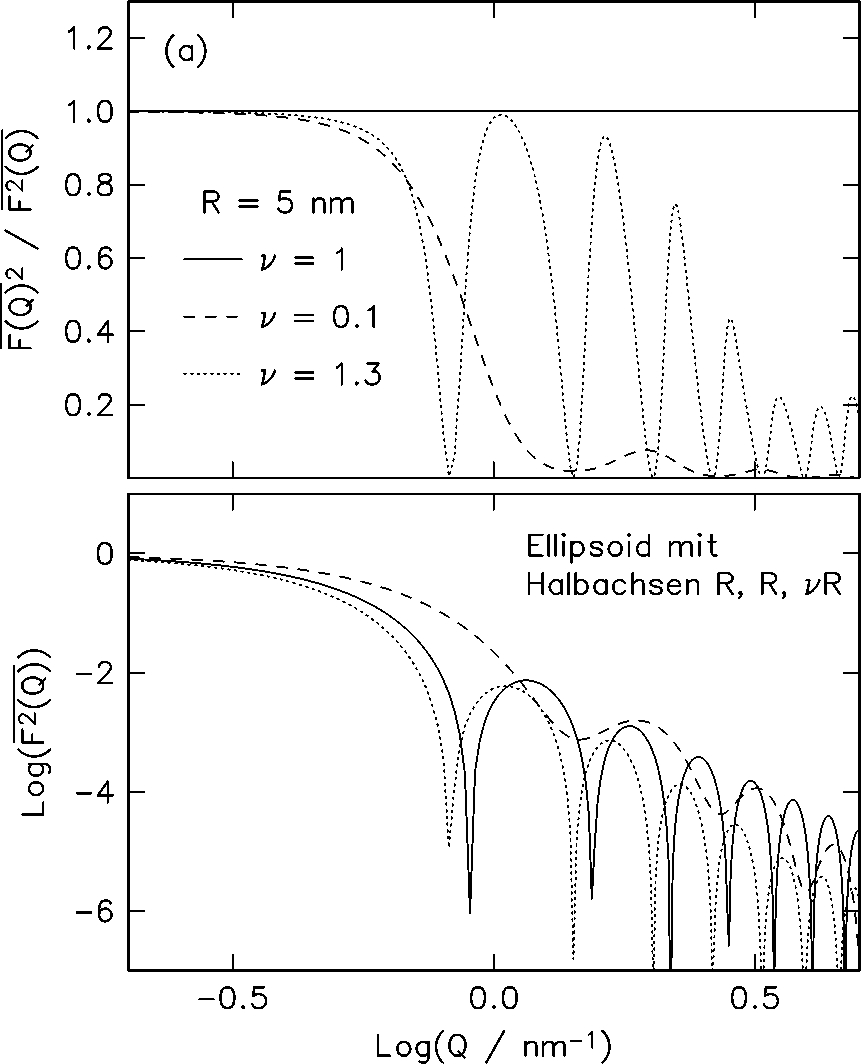
\includegraphics[width=0.48\textwidth,height=0.6\textwidth]{FORMINTE.png}}
\hfill
\subfigure[Influence of a particle size distribution
 ${\rm LogNorm}(R) = \exp\left(-(\ln\mu-\ln R)^2 / (2 \sigma^2)\right)$ of
 the widths  $\sigma$ = 0.1, 0.2, 0.3, 0.4 for $\mu=5$ nm on
$\vert\overline{F(Q)}\vert^2 / \overline{\abs{F(Q)}^2}$.
]{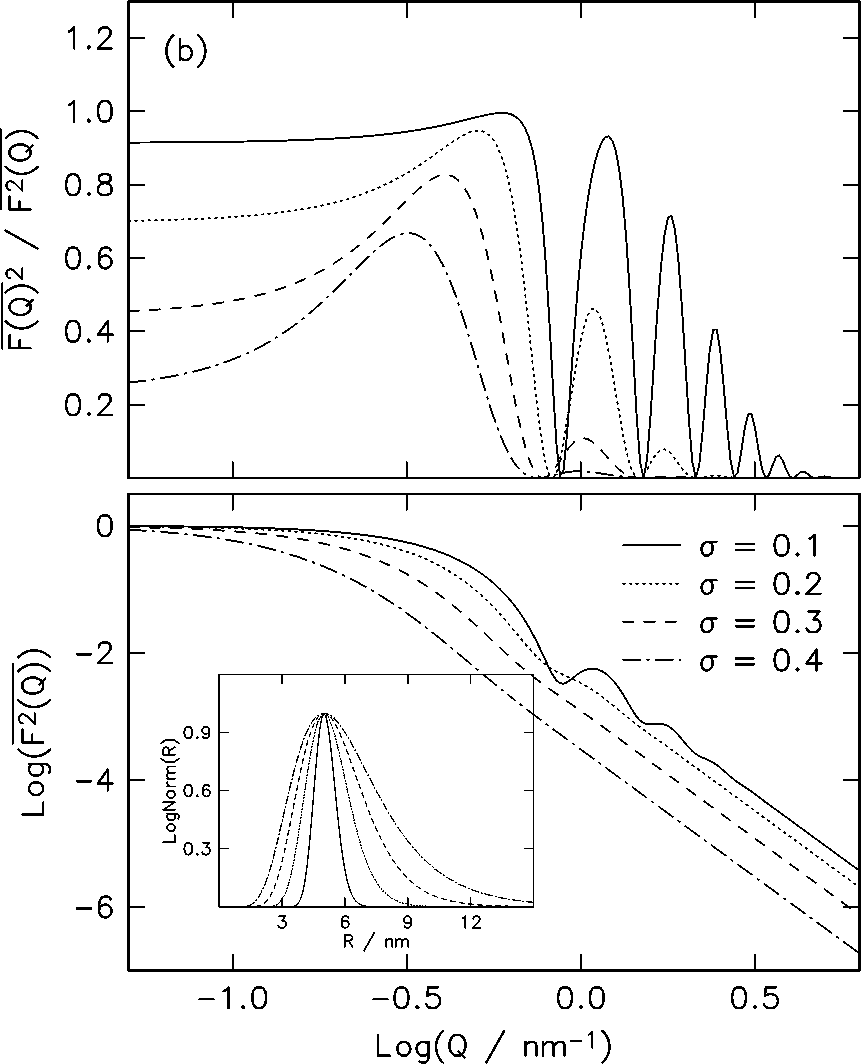
\includegraphics[width=0.48\textwidth,height=0.6\textwidth]{SIZEINTE.png}} \\
\caption{For identical and spherical symmetric scatterers the ratio
$\vert\overline{F(Q)}\vert^2 / \overline{\abs{F(Q)}^2} \equiv 1$.
Interparticle interferences depend then only on the relative positions of
the scatterers. Size distribution  and irregular shapes reduce
these interference effects.}
\label{fig:formfactor:interferenzen}
\end{figure}

\subsection{Scattering laws and structural parameter}

In this section a series of useful scattering laws are presented, which
are useful for a simple analysis of experimental data and which allow an
easy determination of structural parameters.
\cite{book:Guinier:Fournet}.

\subsubsection{Porod volume}

The ratio of the scattering intensity in forward direction $I(Q=0)=N\,
V_P^2\, \Delta\eta^2$ and the scattering invariant  $\tilde Q =
2\pi^2\Delta\eta^2\, V\, f_p(1-f_p)$ can be used to determine the particle volume $V_P$
($V$ describes the illuminated sample volume).
$f_p\, V = N\, V_P$ corresponds to the total volume of all scatterers
whereby the particle volume $V_P$ can be calculated by
\BE
\frac{V_P}{1-f_p} \, \stackrel{f_p \ll 1}{\simeq} \,  V_P
        = 2\pi^2\, \frac{I(Q=0)}{\tilde Q} .
\EE
The measurement of the scattering curve in relative units is therefore sufficiant
to determine the volume of a homogeneous scatterer. Sources of errors for this way
of determination of particle sizes are the extrapolation into forward direction und
more important the extrapolation to large scattering angles
($Q^{-4}$-extrapolation). Furthermore for large volume fractions $f_p$
the particle volume has to be eventually corrected by a prefactor
$1/(1-f_p)$ which is not always known.

\subsubsection{Radius of gyration and Guinier approximation}

The scattering intensity for small angles can be approximated in a series expansion
by replacing the expression $\frac{\sin Qr}{Qr}$ in eq.\ \ref{IQofgamma}
by a McLaurin series which leads to
\BE
I(Q) = V\, \int 4\pi\, r^2\, \gamma(r)\,
       \left[1-\frac{Q^2r^2}{3!} + \frac{Q^4r^4}{5!} - \dots \right] \, dr
       \quad ,
\EE
i.e.\ $I(Q)$ is expanded by moments $\overline{r^n}$ of $\gamma(r)$.
The first term corresponds to the scattering intensity of $Q=0$.
For the second term Guinier and Fournet \cite{book:Guinier:Fournet}
have shown, that it can be related to the gyration radius of the scattering length density
$R_G$ by
\BE
V\,\int 4\pi\, r^2\, \frac{Q^2r^2}{3!}\, \gamma(r)\, dr = I(0)\,
         \frac{Q^2R_G^2}{3}
     \quad \Rightarrow \quad
   I(Q) = I(0) \, \left( 1-\frac{Q^2R_G^2}{3} \right)
\EE
with $R_G^2 = \int \eta(r)\, r^2\, dr/\int \eta(r)\, dr$.
Up to the term of $Q^4$ this series expansion at the beginning of the scattering curve
is identical to the series expansion of an exponential function which than leads to
the well known Guinier approximation
\BE
I(Q) = I(0)\, e^{-Q^2R_G^2/3} .
\label{eq:Guinier}
\EE
The Guinier law is valid for any particle shape which is roughly
isodiametric. For flat or elongated structures the Guinier law has to be
corrected slightly \cite{book:Feigin:Svergun,book:Guinier:Fournet}.
The radius of gyration for a sphere with radius $R$ is given by $R_G=\sqrt{3/5}\, R$.
The Guinier law is valid in the scattering vector interval $0<Q<1/R_G$.

\subsubsection{Correlation length}

Another characteristic quantity, which can be easily extracted from
the scattering curve $I(Q)$ is the correlation length $l_c$. The correlation length
is defined as the average width of the correlation function  $\gamma(r)$:
\BE
l_c = \frac{2}{\gamma(0)}\, \int \gamma(r) \, dr .
\EE
Together with the definition of the scattering invariant $\tilde Q$ in
eq.\  \ref{Invariante} and the relation between $I(Q)$ and $\gamma(r)$ in
eq.\ \ref{gamma} this results after a short calculation (changing of
integrations) to
\BE
l_c = \pi\, \frac{\int Q\, I(Q)\, dQ}{\int Q^2\, I(Q)\, dQ} \quad .
\EE
A sphere with radius $R$ has therefore a correlation length of $l_c = \frac{3}{2}\, R$.

\subsubsection{Porod law and specific surfaces}

The Porod law describes the scattering behavior at large $Q$ values.
As the scattering intensity $I(Q)$ and the correlation function $\gamma(r)$
are related via the Fourier transformation the intensity $I(Q)$ is determined
at large values of $Q$ mainly by $\gamma(r)$ at small $r$. For small $r$  the
correlation function $\gamma(r)$ can be expanded in a Taylor series and one
gets according to Guinier and Fournet \cite{book:Guinier:Fournet}
\BE
\frac{\gamma(r)}{\gamma(0)} = 1 - \frac{1}{4} \, \frac{S}{V} + \dots
\quad ,
\label{eq:gamma:Taylor}
\EE
whereby $S$ is the total surface of all scatterer in the illuminated sample volume $V$.
Eq.\ \ref{eq:gamma:Taylor} together with \ref{IQofgamma} result for large
$Q$ values into the Porod law
\BE
I(Q) \longrightarrow \Delta\eta^2\, \frac{2\pi\, S}{Q^4} .
\label{eq:Porodlaw}
\EE
A scaling of the scattering intensity on $\tilde Q$ provides an expression
for the specific surface $S/V$ of
\BE
\lim_{Q\rightarrow \infty} \, \pi\,\frac{I(Q)}{\tilde Q}\, Q^4\, f_p\,
(1-f_p) = \frac{S}{V} .
\label{eq:spez:surface}
\EE
The Porod law can be applied to all systems having sharp interfaces.
